\documentclass[11pt, a4paper]{article}

% --- PACKAGES ---
\usepackage[utf8]{inputenc}
\usepackage[T1]{fontenc}
\usepackage[dutch]{babel}
\usepackage{amsmath, amssymb, amsfonts} % Math packages
\usepackage{graphicx}           % To include images
\usepackage{geometry}           % Adjust margins
\usepackage[svgnames]{xcolor}    % Color definitions
\usepackage{hyperref}           % Clickable links
\usepackage{csquotes}           % Recommended for biblatex
\usepackage[
    backend=biber,          % Use biber backend
    style=apa,              % APA citation style
    sorting=nyt             % Sort bibliography by name, year, title
]{biblatex}
\usepackage{booktabs}           % Nicer tables
\usepackage{longtable}          % For tables spanning pages
\usepackage{array}              % For advanced column formatting

% --- GEOMETRY ---
\geometry{
    a4paper,
    left=2.5cm,
    right=2.5cm,
    top=2.5cm,
    bottom=2.5cm
}

% --- HYPERREF SETUP ---
\hypersetup{
    colorlinks=true,    % Enable colored links
    linkcolor=Blue,     % Color for internal links (TOC, equations)
    citecolor=Blue,     % Color for citations
    urlcolor=Blue,      % Color for URLs
    pdftitle={Eindopdracht Informatica: Algebraïsche Physics Engine},
    pdfauthor={Joost Koch},
    pdfsubject={Eindopdracht Informatica V6},
    pdfkeywords={Physics Engine, Algebraïsch, Continuous Collision Detection, Event-Based Simulation, Python, Pygame, One More Brick}
}

% --- BIBLIOGRAPHY ---
\addbibresource{references.bib} % Link to your .bib file

% --- MATH COMMANDS (Optional examples) ---
\newcommand{\vect}[1]{\mathbf{#1}}      % Vector notation (bold)
\newcommand{\norm}[1]{\left\lVert#1\right\rVert} % Norm (length) of a vector
\newcommand{\abs}[1]{\left\lvert#1\right\rvert} % Absolute value
\newcommand{\point}[1]{\{#1\}}        % Point notation (e.g., {x, y})

% --- Definities voor tabel kolommen ---
\newcolumntype{L}[1]{>{\raggedright\arraybackslash}p{#1}} % Links uitgelijnd
\newcolumntype{P}[1]{>{\raggedright\arraybackslash}p{#1}} % Paragraaf kolom

% --- DOCUMENT INFO ---
\title{
    \vspace{-1cm} % Move title up slightly
    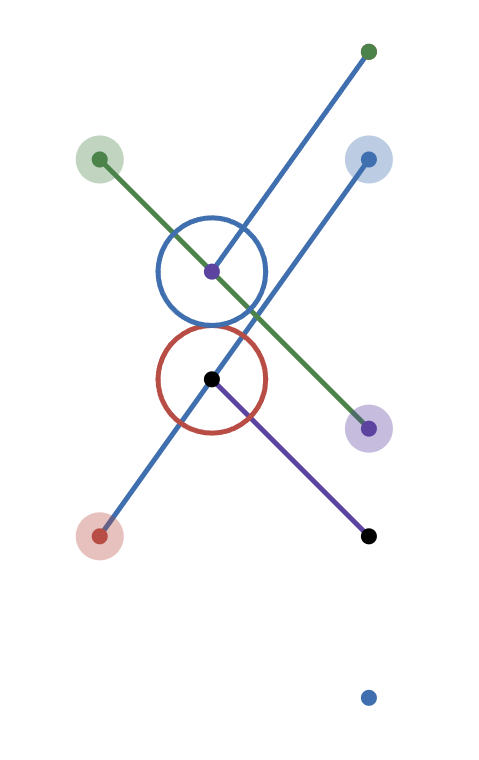
\includegraphics[width=0.8\textwidth]{header-image.png} \\ % Include your header image
    \vspace{0.5cm}
    \textbf{Eindopdracht Informatica V6} \\
    \large Een Algebraïsche 2D Physics Engine zonder Tijdstappen \\
    \normalsize Toegepast in een "One More Brick"-achtige Game
}
\author{Joost Koch \\ Klas V6B \\ Het Amsterdams Lyceum} % School en klas aangepast
\date{April 2025}

% --- BEGIN DOCUMENT ---
\begin{document}

\maketitle
\thispagestyle{empty} % No page number on title page
\newpage

\tableofcontents
\thispagestyle{empty} % No page number on TOC page
\newpage
\setcounter{page}{1} % Start page numbering here

% ===================================================================
\section{Inleiding}
% ===================================================================

\subsection{Motivatie en Onderwerpkeuze}
De keuze voor dit project kwam voort uit een fascinatie voor game physics en de inherente beperkingen van traditionele, op discrete tijdstappen gebaseerde simulaties. Het fenomeen 'tunneling', waarbij snel bewegende objecten door dunne muren kunnen gaan, en de accumulerende onnauwkeurigheden waren specifieke frustraties. Dit leidde tot de ambitie om een physics engine te ontwikkelen die botsingen fundamenteel anders aanpakt: volledig algebraïsch, zonder tijdstappen. De uitdaging lag in het vinden en implementeren van de exacte wiskundige oplossingen voor botsingsmomenten, wat een dieper begrip van zowel wiskunde als programmeren vereist. Het doel was een preciezere en conceptueel robuustere engine, gedemonstreerd in een game zoals "One More Brick", waar nauwkeurige bal-botsingen essentieel zijn.

\subsection{Doelstelling}
Het doel van deze eindopdracht was het ontwikkelen en evalueren van een functionele 2D physics engine in Python die botsingen tussen cirkels en lijnen volledig algebraïsch berekent en afhandelt (event-based), zonder gebruik te maken van discrete tijdstappen. De effectiviteit en precisie van deze engine worden gedemonstreerd door de integratie in een speelbare "One More Brick"-achtige game, ontwikkeld met Pygame. Het project moest binnen de gestelde periode van de eindopdracht (ca. 3 weken effectieve werktijd) worden voltooid.
\newpage
\subsection{De Uitdaging}
De primaire uitdaging van dit project was de overstap van een tijdstap-gebaseerde benadering naar een puur algebraïsche (event-based) simulatie. Dit omvatte:
\begin{itemize}
    \item \textbf{Wiskundige Complexiteit:} Het afleiden, begrijpen en correct implementeren van formules voor het exacte \textit{Time of Impact} (TOI) voor diverse botsingsscenario's (cirkel-lijn, cirkel-eindpunt, cirkel-cirkel).
    \item \textbf{Event Management:} Het ontwerpen van een systeem dat efficiënt de \textit{eerstvolgende} botsing in het gehele systeem kan identificeren en de simulatie exact naar dat moment kan 'vooruitspoelen'.
    \item \textbf{Robuustheid:} Omgaan met floating-point onnauwkeurigheden die kunnen leiden tot gemiste botsingen of objecten die vast komen te zitten.
    \item \textbf{Botsingsafhandeling:} Correct toepassen van natuurkundige principes (zoals reflectie of impulsbehoud) op het exacte moment van impact.
    \item \textbf{Performance:} Balanceren van de computationele kosten van exacte berekeningen met de noodzaak voor een speelbare framerate.
\end{itemize}
Deze aspecten vereisten een dieper begrip van geometrie, analyse en numerieke methoden dan typische game physics implementaties.

\subsection{Leeswijzer}
Dit verslag beschrijft het ontwikkelproces en het eindresultaat van de algebraïsche physics engine. Hoofdstuk \ref{sec:methode} detailleert de gekozen aanpak, de gebruikte technologieën en de kernalgoritmes. Hoofdstuk \ref{sec:product} beschrijft de architectuur en functionaliteiten van zowel de engine als de game. Hoofdstuk \ref{sec:evaluatie} evalueert het product kritisch, inclusief sterktes, zwaktes en een vergelijking met traditionele methoden. Hoofdstuk \ref{sec:problemen} bespreekt de ondervonden uitdagingen en de gevonden oplossingen. Hoofdstuk \ref{sec:conclusie} vat de resultaten samen en reflecteert op het leerproces. De gebruikte bronnen zijn te vinden in de bibliografie. Een samenvatting van het logboek is te vinden in Sectie \ref{sec:logboek}. % Aangepast om naar nieuwe sectie te verwijzen
\newpage
% ===================================================================
\section{Methode van Aanpak} \label{sec:methode}
% ===================================================================

\subsection{Concept: Algebraïsche (Event-Based) Simulatie}
In tegenstelling tot traditionele physics engines die de toestand van objecten bijwerken met een vaste, kleine tijdstap $\Delta t$ (bijv. $\vect{p}_{new} = \vect{p}_{old} + \vect{v} \cdot \Delta t$), hanteert deze engine een \textit{event-based} aanpak \parencite{PrincetonEventSim}. De simulatie springt direct van de ene significante gebeurtenis (meestal een botsing) naar de volgende:
\begin{enumerate}
    \item \textbf{Voorspel TOI:} Voor elk relevant paar interacterende objecten (bal-lijn, bal-bal), bereken algebraïsch het \textit{Time of Impact} ($t_{impact}$), het exacte tijdstip in de toekomst waarop een botsing zou plaatsvinden als hun huidige beweging ongestoord doorgaat.
    \item \textbf{Vind Eerste Event:} Bepaal de minimale $t_{impact}$ over alle mogelijke botsingen in het systeem. Dit is de tijd tot de eerstvolgende gebeurtenis, $t_{min}$.
    \item \textbf{Vooruitspoelen:} Verplaats \textit{alle} objecten in het systeem exact $t_{min}$ vooruit in de tijd naar hun posities op het moment van deze eerste botsing: $\vect{p}_{new} = \vect{p}_{old} + \vect{v} \cdot t_{min}$.
    \item \textbf{Handel Event Af:} Pas de snelheden aan van de objecten die betrokken zijn bij de botsing(en) die plaatsvinden op $t_{min}$.
    \item \textbf{Update Voorspellingen:} Herbereken de potentiële TOI's voor de objecten die zojuist gebotst zijn (en objecten waarmee zij nu mogelijk gaan botsen), aangezien hun snelheden zijn veranderd.
    \item \textbf{Herhaal:} Ga terug naar stap 2.
\end{enumerate}
Deze methode, ook bekend als \textit{Continuous Collision Detection} (CCD) \parencite{Box2DDocs, CattoCCD}, garandeert dat geen botsingen worden gemist, ongeacht de snelheid van objecten.

\subsection{Gebruikte Technologieën}
\begin{itemize}
    \item \textbf{Programmeertaal:} Python 3.
    \item \textbf{Bibliotheken:}
        \begin{itemize}
            \item \texttt{NumPy} \parencite{NumPy}: Essentieel voor efficiënte vector- en matrixberekeningen die de basis vormen van de geometrische en wiskundige operaties.
            \item \texttt{Pygame} \parencite{Pygame}: Gebruikt voor het creëren van het game window, het tekenen van de simulatie (visualisatie), en het afhandelen van gebruikersinvoer (muis, toetsenbord).
            \item \texttt{math}: Standaard Python library voor basale wiskundige functies zoals $\sqrt{\cdot}$.
        \end{itemize}
\end{itemize}
\newpage
\subsection{Data Structuur en Klassen}
De code is modulair opgezet:
\begin{itemize}
    \item \texttt{data\_types.py}: Bevat de fundamentele klassen \texttt{Point}, \texttt{Vector}, en \texttt{Line}, die de geometrische basis vormen en gebruikmaken van NumPy arrays.
    \item \texttt{oneMoreBrickEngine.py}: De kern van de physics engine.
        \begin{itemize}
            \item \texttt{MovingObject}, \texttt{Ball}: Representeren objecten met positie $\vect{p}$, snelheid $\vect{v}$, en (voor \texttt{Ball}) radius $r$.
            \item \texttt{Collision}: Data container voor een gedetecteerde botsing (betrokken bal, botsingspunt, raakpunt, type, etc.). Cruciaal is de \texttt{time\_left} eigenschap.
            \item \texttt{BallLineInteraction}, \texttt{BallBallInteraction}: Klassen die de complexe logica bevatten voor het \textit{berekenen} van de TOI voor specifieke interactietypes (zie Sectie \ref{ssec:kernalgoritmes}).
            \item \texttt{PhysicsEnvironment}: Orkestreert de simulatie. Beheert lijsten van objecten (\texttt{objects}) en statische structuren (\texttt{lines}, \texttt{collision\_objects}). De \texttt{run\_tick} methode implementeert de event-based loop.
        \end{itemize}
    \item \texttt{oneMoreBrickGame.py}: Implementeert de specifieke game.
        \begin{itemize}
            \item \texttt{GridCell}, \texttt{GameGrid}: Representeert het speelveld met blokken en power-ups.
            \item \texttt{GameBall}, \texttt{PowerupBall}, \texttt{CollisionBall}: Spelspecifieke subklassen van \texttt{Ball} met extra eigenschappen.
            \item \texttt{Renderer}: Verantwoordelijk voor het tekenen van de game state m.b.v. Pygame.
            \item \texttt{Game}: Hoofdklasse van de applicatie, beheert spelverloop, levels, interactie tussen speler, engine en renderer.
        \end{itemize}
    \item \texttt{grid\_utils.py}: Hulpfuncties om het discrete \texttt{GameGrid} om te zetten naar continue \texttt{Line} objecten voor de physics engine.
\end{itemize}
\newpage
\subsection{Kernalgoritmes: Berekenen van Time of Impact (TOI)} \label{ssec:kernalgoritmes}

\subsubsection{Bal-Lijn Interactie}
De interactie tussen een bal (centrum $\vect{p}_b$, snelheid $\vect{v}_b$, radius $r$) en een statisch lijnsegment $\vect{L}$ (eindpunten $\vect{L}_1, \vect{L}_2$) wordt berekend in \texttt{BallLineInteraction}. Een botsing kan optreden met de eindpunten of het lijnsegment zelf.

\paragraph{Botsing met Eindpunt $\vect{E}$:} We zoeken $t \ge 0$ waarvoor de afstand tussen het balcentrum op tijd $t$, $\vect{p}_b(t) = \vect{p}_b + \vect{v}_b t$, en het eindpunt $\vect{E}$ gelijk is aan $r$:
\[ \norm{\vect{p}_b(t) - \vect{E}}^2 = r^2 \]
\[ \norm{(\vect{p}_b - \vect{E}) + \vect{v}_b t}^2 = r^2 \]
Uitwerken via het dot product $(\vect{a}+\vect{b}) \cdot (\vect{a}+\vect{b}) = \vect{a}\cdot\vect{a} + 2\vect{a}\cdot\vect{b} + \vect{b}\cdot\vect{b}$ levert een kwadratische vergelijking $At^2 + Bt + C = 0$:
\begin{align*}
    A &= \vect{v}_b \cdot \vect{v}_b = \norm{\vect{v}_b}^2 \\
    B &= 2 (\vect{p}_b - \vect{E}) \cdot \vect{v}_b \\
    C &= \norm{\vect{p}_b - \vect{E}}^2 - r^2
\end{align*}
De kleinste niet-negatieve oplossing $t$ (indien $\Delta = B^2 - 4AC \ge 0$) is een potentiële TOI.

\paragraph{Botsing met Lijnsegment:} Het vinden van het moment waarop de bal het lijnsegment raakt, is complexer. De code lijkt een methode te gebruiken die de dichtstbijzijnde punten berekent (zie \texttt{Line.closest\_point}) en vervolgens via de afstand tot de bewegingslijn van de bal de $t$ bepaalt waarbij de afstand tot het lijnstuk of eindpunt $r$ wordt \parencite{LeongCircleLine, FeronatoCircleLine}. Cruciaal is de check of het dichtstbijzijnde punt op de (oneindige) lijn ook daadwerkelijk \textit{op het segment} $\vect{L}_1\vect{L}_2$ ligt.

De kleinste geldige $t \ge 0$ van alle scenario's (eindpunt 1, eindpunt 2, lijnsegment) is de TOI voor deze interactie.

\subsubsection{Bal-Bal Interactie}
Voor twee ballen (Bal 1: $\vect{p}_1, \vect{v}_1, r_1, m_1$; Bal 2: $\vect{p}_2, \vect{v}_2, r_2, m_2$) zoeken we $t \ge 0$ waarvoor de afstand tussen de centra gelijk is aan $r = r_1 + r_2$. De posities op tijd $t$ zijn $\vect{p}_1(t) = \vect{p}_1 + \vect{v}_1 t$ en $\vect{p}_2(t) = \vect{p}_2 + \vect{v}_2 t$.
De botsingsvoorwaarde is $\norm{\vect{p}_2(t) - \vect{p}_1(t)}^2 = r^2$.
Definieer relatieve positie $\vect{p}_{rel} = \vect{p}_2 - \vect{p}_1$ en relatieve snelheid $\vect{v}_{rel} = \vect{v}_2 - \vect{v}_1$. De voorwaarde wordt:
\[ \norm{\vect{p}_{rel} + \vect{v}_{rel} t}^2 = r^2 \]
Dit leidt weer tot de kwadratische vergelijking $At^2 + Bt + C = 0$ \parencite{ToptalPhysics, LeongCircleCircle, DesmosBallBall}:
\begin{align*}
    A &= \vect{v}_{rel} \cdot \vect{v}_{rel} = \norm{\vect{v}_{rel}}^2 \\
    B &= 2 \vect{p}_{rel} \cdot \vect{v}_{rel} \\
    C &= \vect{p}_{rel} \cdot \vect{p}_{rel} - r^2 = \norm{\vect{p}_{rel}}^2 - r^2
\end{align*}
Deze coëfficiënten $A, B, C$ komen overeen met de implementatie in \texttt{BallBallInteraction.calc\_collisions} en de Desmos-visualisatie \parencite{DesmosBallBall}. De kleinste niet-negatieve oplossing $t = \frac{-B - \sqrt{B^2 - 4AC}}{2A}$ (indien $B^2 - 4AC \ge 0$) is de TOI.

\subsubsection{Botsingsafhandeling (Response)}
Op het moment $t_{min}$ worden snelheden aangepast.
\paragraph{Bal-Lijn:} De snelheid $\vect{v}_b$ wordt gereflecteerd t.o.v. de normaal $\vect{N}$ van het botsingsoppervlak: $\vect{v}_{new} = \vect{v}_{old} - 2 \operatorname{proj}_{\vect{N}}(\vect{v}_{old}) = \vect{v}_{old} - 2 \frac{\vect{v}_{old} \cdot \vect{N}}{\norm{\vect{N}}^2} \vect{N}$. De implementatie in \texttt{Collision.calc\_new\_vel} berekent de nieuwe snelheid gebaseerd op de reflectie van het centrum t.o.v. het raakpunt. Een factor \texttt{collision\_efficiency} wordt toegepast.
\paragraph{Bal-Bal:} Voor elastische botsingen wordt impuls behouden. De snelheidsverandering vindt plaats langs de normaalvector $\vect{n} = \operatorname{normalize}(\vect{p}_2(t_{min}) - \vect{p}_1(t_{min}))$. De formules voor de nieuwe snelheden $\vect{w}_1, \vect{w}_2$ in de code (\texttt{BallBallInteraction.calc\_new\_vels}) lijken gebaseerd op \parencite{LeongCircleCircle}, maar de exacte afleiding vereist verificatie:
\begin{align*}
    \vect{p} &= (\vect{v}_1 \cdot \vect{n}) \vect{n} - (\vect{v}_2 \cdot \vect{n}) \vect{n} \quad \text{(Gerelateerd aan relatieve normaal-snelheid)} \\
    \vect{w}_1 &= \vect{v}_1 + \norm{\vect{p}} \vect{n} \quad \text{(Let op: teken + ongebruikelijk?)} \\
    \vect{w}_2 &= \vect{v}_2 - \norm{\vect{p}} \vect{n} \quad \text{(Let op: teken - ongebruikelijk?)}
\end{align*}
Standaard impuls formules \parencite{DesmosBallBall} zijn: $j = \frac{-2(\vect{v}_1 - \vect{v}_2)\cdot\vect{n}}{1/m_1 + 1/m_2}$, $\vect{w}_1 = \vect{v}_1 + j/m_1 \vect{n}$, $\vect{w}_2 = \vect{v}_2 - j/m_2 \vect{n}$. De implementatie gebruikt $m_1=m_2=1$ (impliciet) en een mogelijk vereenvoudigde of andere impulsberekening.

\newpage
% ===================================================================
\section{Het Product: Engine \& Game}
\label{sec:product}
% ===================================================================

\subsection{Architectuur Overzicht}
Het product bestaat uit twee hoofdcomponenten: de herbruikbare, generieke \texttt{oneMoreBrickEngine.py} en de specifieke game-implementatie \texttt{oneMoreBrickGame.py}. De \texttt{Game} klasse gebruikt een instantie van \texttt{PhysicsEnvironment} om de fysica te simuleren en een \texttt{Renderer} om de staat te visualiseren. Data types zijn gescheiden in \texttt{data\_types.py} en grid-conversie in \texttt{grid\_utils.py}.

\subsection{Functionaliteiten Physics Engine}
\begin{itemize}
    \item Algebraïsche (event-based) simulatie zonder tijdstappen.
    \item Continue botsingsdetectie (CCD) en exacte TOI-berekening voor:
        \begin{itemize}
            \item Bewegende cirkel vs. statisch lijnsegment (incl. eindpunten).
            \item Bewegende cirkel vs. bewegende cirkel.
            \item Bewegende cirkel vs. statische cirkel (gebruikt voor power-ups/obstacles).
        \end{itemize}
    \item Elastische botsingsafhandeling (reflectie/impuls-gebaseerd).
    \item Beheer van meerdere dynamische \texttt{Ball} objecten.
    \item Beheer van statische \texttt{Line} objecten en \texttt{collision\_objects}.
    \item Identificatie en afhandeling van het eerstvolgende event in het systeem.
    \item Optionele functionaliteiten: zwaartekracht, instelbare botsingsefficiëntie.
    \item Mechanisme voor het corrigeren van kleine overlappingen (\texttt{fix\_clipping}).
\end{itemize}

\subsection{Functionaliteiten Game ("One More Brick Clone")}
\begin{itemize}
    \item Grid-gebaseerd speelveld (\texttt{GameGrid}).
    \item Vernietigbare blokken met levenspunten (\texttt{GridCell.value}).
    \item Diverse blokvormen (vierkant, driehoeken - type 1-5).
    \item Vaste cirkelvormige obstakels (type 6).
    \item Power-ups met diverse effecten (extra bal, laserlijnen, etc. - type < 0).
    \item Richt- en schietmechanisme voor ballen vanuit een vast punt.
    \item Level progressie: nieuwe rij blokken/power-ups per ronde.
    \item Game over conditie (blokken bereiken onderkant).
    \item Visuele feedback en interactie via Pygame (\texttt{Renderer}).
    \item Checkpoint systeem gebaseerd op volledig legen van het veld.
\end{itemize}

% ===================================================================
\section{Evaluatie} \label{sec:evaluatie}
% ===================================================================

\subsection{Mogelijkheden en Sterke Punten}
\begin{itemize}
    \item \textbf{Precisie:} Het grootste voordeel. Botsingen worden exact berekend en afgehandeld op het correcte moment, waardoor 'tunneling' effectief wordt geëlimineerd, zelfs bij hoge snelheden. Dit is cruciaal voor de beoogde game.
    \item \textbf{Determinisme:} Gegeven dezelfde initiële condities en input, levert de simulatie altijd exact hetzelfde resultaat, wat testen en debuggen vergemakkelijkt.
    \item \textbf{Stabiliteit:} De event-based aanpak is inherent stabieler dan tijdstap-methoden die kunnen exploderen bij grote stappen of stijve interacties.
    \item \textbf{Conceptuele Correctheid:} De methode modelleert de fysica op een fundamenteler niveau (continue tijd) dan discrete benaderingen.
\end{itemize}

\subsection{Beperkingen en Zwakke Punten}
\begin{itemize}
    \item \textbf{Performance:} Het berekenen van alle paarsgewijze TOI's kan computationeel intensief zijn. Zonder optimalisaties zoals spatial partitioning, schaalt de complexiteit voor $n$ objecten naar $O(n^2)$ voor object-object interacties. Dit kan merkbaar worden bij een zeer groot aantal ballen of complexe levels.
    \item \textbf{Complexiteit Implementatie:} De wiskunde en de logica van de event-loop zijn aanzienlijk complexer dan een eenvoudige tijdstap-integrator.
    \item \textbf{Floating-Point Gevoeligheid:} Ondanks de exacte aanpak, blijft de implementatie gevoelig voor afrondingsfouten in floating-point getallen. Dit kan leiden tot 'bijna'-botsingen die net wel of net niet gedetecteerd worden, of kleine overlappingen na een botsing. De noodzaak voor \texttt{fix\_clipping} bevestigt dit.
    \item \textbf{Uitbreidbaarheid:} Het toevoegen van complexere fysica (rotatie, frictie, complexere vormen zoals polygonen) is significant moeilijker in een puur algebraïsche/event-based engine dan in een tijdstap-engine waar benaderingen makkelijker toe te passen zijn.
    \item \textbf{Bal-Bal Realisme:} De huidige botsingsafhandeling lijkt vereenvoudigd (zie Sectie \ref{ssec:kernalgoritmes}). Voor perfect realisme is correcte impuls- en energiebehoud met massa vereist.
\end{itemize}

\subsection{Vergelijking met Tijdstap-gebaseerde Engines}
\begin{table}[h]
\centering
\caption{Vergelijking Algebraïsch vs. Tijdstap}
\label{tab:vergelijking}
\begin{tabular}{@{}lll@{}}
\toprule
Aspect             & Algebraïsch (Event-Based)                    & Tijdstap-gebaseerd                        \\ \midrule
Precisie           & Hoog (exact TOI)                             & Beperkt (afhankelijk van $\Delta t$)      \\
Tunneling          & Geen                                         & Mogelijk bij hoge snelheid / kleine $\Delta t$ \\
Stabiliteit        & Hoog                                         & Kan instabiel worden                      \\
Complexiteit Impl. & Hoog (wiskunde, event loop)                & Lager (integratie formules)             \\
Performance ($n$ obj.) & Potentieel $O(n \log n)$ - $O(n^2)$      & Vaak sneller voor veel obj. (benadering) \\
Uitbreidbaarheid   & Moeilijker (complexe fysica)                 & Makkelijker (benaderingen toevoegen)      \\ \bottomrule
\end{tabular}
\end{table}
De algebraïsche aanpak is superieur waar absolute precisie en stabiliteit vereist zijn (zoals in deze game), maar inferieur waar performance bij zeer veel objecten of de eenvoud van implementatie de doorslag geeft \parencite{CollisionDetectionWiki}.

\subsection{Voldoet het Product aan de Doelstelling?}
Ja, het ontwikkelde product voldoet aan de gestelde doelstelling. Er is een functionele 2D physics engine gerealiseerd die botsingen algebraïsch berekent zonder discrete tijdstappen. Deze engine is succesvol geïntegreerd in een speelbare "One More Brick"-achtige game die de precisie van de engine demonstreert. De kernuitdagingen van de algebraïsche aanpak zijn aangegaan en geïmplementeerd.

% ===================================================================
\section{Ondervonden Problemen en Oplossingen} \label{sec:problemen}
% ===================================================================
Gedurende het project (zie logboek in Sectie \ref{sec:logboek}) kwamen diverse uitdagingen naar voren:

\begin{itemize}
    \item \textbf{Wiskundige Hürden:} Het correct afleiden en implementeren van de TOI-formules, met name voor bal-bal interactie, was complex.
        \textit{Oplossing:} Grondig online onderzoek (o.a. \parencite{LeongCircleLine, LeongCircleCircle, ToptalPhysics}), gebruik van visualisaties zoals Desmos \parencite{DesmosBallBall} ter verificatie, en stapsgewijze implementatie en testen.
    \item \textbf{Floating-Point Precisie Issues:} Kleine afrondingsfouten zorgden soms voor onverwacht gedrag, zoals ballen die 'vast' leken te zitten of net door objecten heen gingen na een berekende botsing.
        \textit{Oplossing:} Implementatie van de \texttt{fix\_clipping} routine die na elke stap controleert op overlapping en objecten fysiek uit elkaar duwt. Gebruik van \texttt{math.isclose} waar mogelijk in plaats van exacte gelijkheidstests.
    \item \textbf{Event Management Complexiteit:} Het correct beheren van de 'wachtrij' van toekomstige botsingen en het updaten ervan na elke afgehandelde botsing was een uitdaging.
        \textit{Oplossing:} Implementatie van de \texttt{run\_tick} loop die iteratief de eerstvolgende actie (kleinste \texttt{time\_left}) selecteert, afhandelt, en de lijst van \texttt{collisions} bijwerkt door relevante nieuwe TOI's te berekenen en oude/ongeldige te verwijderen. De \texttt{collisions\_per\_ball} limiet voorkomt oneindige loops.
    \item \textbf{Debugging:} Het vinden van de oorzaak van incorrect gedrag in een event-based systeem is lastig, omdat de simulatietijd niet lineair verloopt.
        \textit{Oplossing:} Intensief gebruik van visuele debugging in Pygame (tekenen van voorspelde paden, botsingspunten) en gerichte print statements. Testen met minimale, controleerbare scenario's.
\end{itemize}

% ===================================================================
\section{Logboek} \label{sec:logboek}
% ===================================================================

\subsection*{Uitgevoerde Activiteiten (Per Dag)}

% \begin{center} % Verwijderd voor longtable
\begin{longtable}{@{} l L{2cm} L{1.5cm} P{6.5cm} @{}}
\caption{Logboek Uitgevoerde Activiteiten (Per Dag)}\label{tab:logboek_long}\\
\toprule
\textbf{Datum} & \textbf{Waar} & \textbf{Tijd (Ca.)} & \textbf{Activiteit \& Reflectie (STARR - Vul aan!)} \\ % Corrected &
\midrule
\endfirsthead

\multicolumn{4}{c}%
{{\bfseries Tabel \thetable\ vervolg}} \\
\toprule
\textbf{Datum} & \textbf{Waar} & \textbf{Tijd (Ca.)} & \textbf{Activiteit \& Reflectie} \\ % Corrected &
\midrule
\endhead

\midrule
\multicolumn{4}{r}{{\textit{Vervolg op volgende pagina}}} \\
\bottomrule
\endfoot

\bottomrule
\endlastfoot

% --- LOGBOEK ENTRIES ---
19-Mar-2025 & Thuis/School & 0.5u & Start project, onderwerp brainstormen. \\
20-Mar-2025 & Thuis/School & 0.5u & Onderwerp verder overwegen, globale aanpak. \\
21-Mar-2025 & Thuis/School & 0.5u & Definitieve keuze algebraïsch, ruwe planning. \\
22-Mar-2025 & Thuis/School & 0.5u & Planning verfijnen, nadenken over eerste stappen. \\
23-Mar-2025 & Thuis/School & 0.5u & Benodigde technologieën/libraries checken. \\
24-Mar-2025 & -            & 0u   & (Geen activiteit) \\
25-Mar-2025 & -            & 0u   & (Geen activiteit) \\
\midrule % Visuele scheiding na brainstorm week
26-Mar-2025 & Thuis        & 1u   & Diepgaand onderzoek algebraïsche botsingen (CCD, TOI), bronnen verzamelen. \\
27-Mar-2025 & Thuis        & 1u   & Onderzoek vervolgen, links/tutorials (Leong, Toptal) bekijken. \\
28-Mar-2025 & Thuis        & 1u   & Implementatie Data Types (\texttt{Point}, \texttt{Vector}, \texttt{Line}) met NumPy, basis tests. \\
29-Mar-2025 & Thuis        & 1u   & Wiskunde Bal-Lijn: afleiden/controleren kwadratische vergelijking eindpunt botsing. \\
30-Mar-2025 & Thuis        & 0.5u   & Wiskunde Bal-Lijn: aanpak lijnsegment botsing uitwerken. Start implementatie \texttt{BallLineInteraction}. \\
31-Mar-2025 & Thuis        & 1.5u & Afronden \texttt{BallLineInteraction} (\texttt{calc\_collisions}, \texttt{calc\_new\_vel}), testen met simpele gevallen (horizontale/verticale lijn). \\
\midrule % Visuele scheiding
01-Apr-2025 & Thuis        & 1.5u & Wiskunde Bal-Bal: Analyseren Desmos-link \parencite{DesmosBallBall}, relatie met kwadratische formule \texttt{t} en impuls/snelheidsformules (\texttt{w1},\texttt{w2}) begrijpen. \\
\textbf{02-Apr-2025} & \textbf{Mediatheek} & \textbf{1u 40m} & \textbf{Implementatie} \texttt{BallBallInteraction}: Code schrijven voor \texttt{calc\_collisions} en \texttt{calc\_new\_vels}. \textbf{Testen:} Direct getest in simpele Pygame-opzet. \textbf{Reflectie:} Efficiënt gewerkt tijdens lesuren, basis werkt. \\
03-Apr-2025 & Thuis        & 1.5u & Implementatie \texttt{PhysicsEnvironment}: Opzet \texttt{run\_tick} loop, \texttt{active\_actions} logica, \texttt{travelled\_time} beheer. \\
04-Apr-2025 & Thuis        & 1.5u & Integratie Pygame: \texttt{Renderer} klasse opzetten, basis visualisatie van ballen en lijnen uit de engine. \\
05-Apr-2025 & Thuis        & 0.5u   & Game Logic: \texttt{Game} klasse, \texttt{GameGrid}/\texttt{GridCell}, \texttt{grid\_utils} gebruiken om lijnen te genereren, basis game state. \\
06-Apr-2025 & Thuis        & 1.5u & Game Logic: Power-up types definiëren en logica in \texttt{register\_collision} toevoegen, level progressie (nieuwe rij). \\
07-Apr-2025 & Thuis & 1u   & Testen \& Debuggen: Game spelen, randgevallen zoeken (botsingen hoeken, snelle ballen), \texttt{fix\_clipping} nalopen, bugs oplossen. \\ % Corrected &
08-Apr-2025 & Thuis        & 1u   & Schrijven Verslag: Hoofdstuk 1 (Inleiding), Hoofdstuk 2 (Methode), focus op gedetailleerde uitleg kernalgoritmes (Sectie 2.4). \\
09-Apr-2025 & Thuis & 1u   & Schrijven Verslag: Hoofdstuk 3 (Product), 4 (Evaluatie), 5 (Problemen), 6 (Conclusie). Logboek opschonen en reflecties aanvullen. \\
10-Apr-2025 & Thuis & 0.5u & Afronden: Laatste checks verslag/logboek, PDF genereren, ZIP maken, inleveren. \\
\midrule
\multicolumn{2}{@{}l}{\textbf{Totaal Geschat:}} & \textbf{~20u} & \\

\end{longtable}
% \end{center} % Verwijderd voor longtable

\newpage
% ===================================================================
\section{Conclusie} \label{sec:conclusie}
% ===================================================================

\subsection{Samenvatting Resultaten}
Deze eindopdracht heeft succesvol geresulteerd in de ontwikkeling van een 2D physics engine die fundamenteel verschilt van traditionele methoden door botsingen volledig algebraïsch en event-based af te handelen. De engine berekent exacte botsingstijden (TOI) voor interacties tussen cirkels en lijnen, waardoor problemen zoals 'tunneling' worden voorkomen. De functionaliteit en precisie zijn gedemonstreerd in een werkende "One More Brick"-achtige game.

\subsection{Belangrijkste Leerpunten}
Dit project was een waardevolle leerervaring op meerdere vlakken:
\begin{itemize}
    \item \textbf{Toegepaste Wiskunde:} Diepgaand begrip en toepassing van lineaire algebra, geometrie en analyse voor het oplossen van concrete fysische problemen (botsingsdetectie en -afhandeling).
    \item \textbf{Algoritmisch Denken:} Ontwerpen en implementeren van complexe algoritmes zoals de event-based simulatie loop en TOI-berekeningen.
    \item \textbf{Software Engineering:} Modulaire code schrijven (scheiding engine/game), gebruik van libraries (NumPy, Pygame), versiebeheer (impliciet), en systematisch debuggen.
    \item \textbf{Physics Engines:} Inzicht verkregen in de fundamentele werking, voordelen en nadelen van zowel event-based als tijdstap-gebaseerde simulaties.
    \item \textbf{Zelfstandigheid en Probleemoplossing:} Het succesvol doorlopen van het project vereiste doorzettingsvermogen, zelfstandig onderzoek en het overwinnen van technische en wiskundige uitdagingen.
\end{itemize}

\subsection{Toekomstige Verbeteringen}
Hoewel het project succesvol was, zijn er diverse mogelijkheden voor uitbreiding:
\begin{itemize}
    \item Implementeren van rotatie voor objecten.
    \item Toevoegen van frictie en luchtweerstand.
    \item Ondersteuning voor complexere vormen (bijv. polygonen via Separating Axis Theorem aangepast voor CCD).
    \item Performance optimalisatie door middel van spatial partitioning (bijv. een grid of quadtree specifiek voor event prediction).
    \item Implementeren van meer realistische bal-bal botsingen gebaseerd op massa en correct impulsbehoud.
    \item Verdere uitbreiding van de game features.
\end{itemize}

\newpage
% ===================================================================
% \section*{Referenties} % APA Stijl heading
% ===================================================================
\printbibliography[heading=bibintoc, title={}] % Print bibliography, add to TOC

\end{document}
% --- END OF DOCUMENT ---